\documentclass[border=2pt]{standalone}
\usepackage{tikz}
\usetikzlibrary{quotes,angles}
\usepackage{amsmath}
\usepackage{amssymb}

\begin{document}

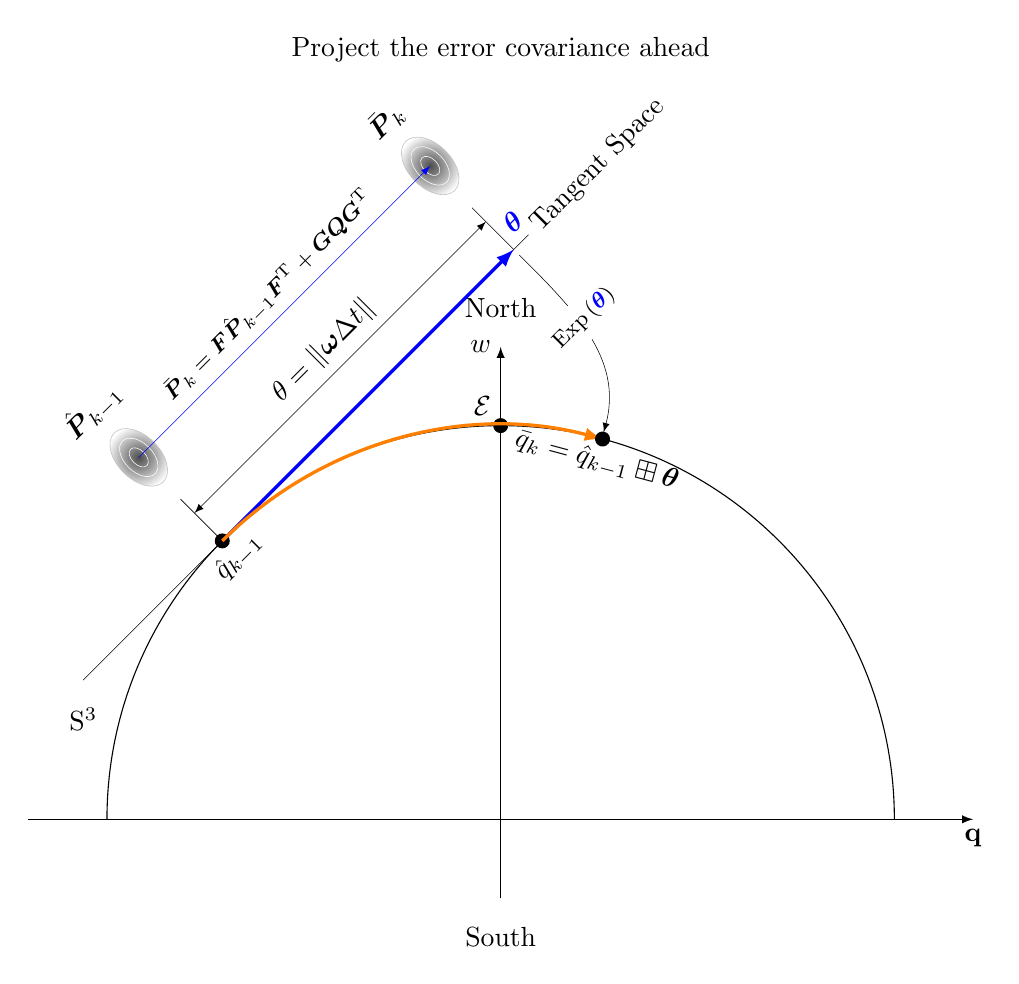
\begin{tikzpicture}[scale=5]

% Draw x and y axis lines
\draw [->,>=latex] (-1.2,0) -- (1.2,0) node [below] {$\mathbf{q}$};
\draw [->,>=latex] (0,-0.2) -- (0,1.2) node [left] {$w$};
\node [above] at (0, 1.25) {North};
\node [below] at (0,-0.25) {South};
\node[above left] at (-1.0,0.2) {$\mathrm{S}^{3}$};
\node[above] at (0.0,1.9) {Project the error covariance ahead};

% Draw a arc at the origin of radius 1
\draw (1,0) arc (000:180:1);
\filldraw[black] (0,1) circle (0.5pt) node[above left ] {$\mathcal{E}$} ;

\begin{scope} [rotate=45]

\filldraw[black] (0.0,1.0) circle (0.5pt) node[below, rotate=45 ] {$\hat{q}_{k-1}$} ;
\draw [very thin] (-.5, 1) -- ( 1.1, 1) node[right, rotate=45] {Tangent Space} ;
\draw [very thick, ->, >=latex, blue] (0,1) -- (1.047,1) node[above right, rotate=45] {$\boldsymbol{\theta}$} ;

\draw [<->,>=latex] [very thin] (0.00, 1.1) -- node[above, rotate=45] {$\theta = \left\Vert \boldsymbol{\omega}\Delta t \right\Vert$} (1.047, 1.1) ;
\draw [very thin] (0.00, 1.00) -- (0.00, 1.15) ;
\draw [very thin] (1.047, 1.00) -- (1.047, 1.15) ;

\draw [->,>=latex] [very thick, orange] (0,1) arc (90:30:1);

% 0.8660 , 0.5000
\draw [->,>=latex] [very thin] (1.047,0.98) to [out=270,in=30] (0.88,0.51) ;
\node [fill=white, rotate=45] at (1.05,0.75) {\footnotesize$\mathrm{Exp}\left( \color{blue}\boldsymbol{\theta}\color{black} \right)$} ;

\begin{scope} [shift={(0.0, 1.3)}, scale=0.08]

% FIXME: 程序有BUG,旋转之后灰度边缘不对。
\draw [very thin, lightgray, inner color=black!70, outer color=black!0] (0,0) ellipse (0.68 and 1.1);
\draw [very thin, lightgray!0] (0,0) ellipse (0.68/3*2 and 1.1/3*2); % \sigma = +-2
\draw [very thin, lightgray!0] (0,0) ellipse (0.68/3   and 1.1/3  ); % \sigma = +-1

\end{scope}

\node[above, rotate=45] at (0.0,1.4) {$\hat{\boldsymbol{P}}_{k-1}$};

\begin{scope} [shift={(1.047, 1.3)}, scale=0.08]

% FIXME: 程序有BUG,旋转之后灰度边缘不对。
\draw [very thin, lightgray, inner color=black!70, outer color=black!0] (0,0) ellipse (0.68 and 1.1);
\draw [very thin, lightgray!0] (0,0) ellipse (0.68/3*2 and 1.1/3*2); % \sigma = +-2
\draw [very thin, lightgray!0] (0,0) ellipse (0.68/3   and 1.1/3  ); % \sigma = +-1

\end{scope}

\node[above, rotate=45] at (1.047,1.4) {$\bar{\boldsymbol{P}}_{k}$};

\draw [very thin, ->,>=latex, color=blue] (0.0, 1.3) -- node[above, rotate=45] {\footnotesize$\color{black}\bar{\boldsymbol{P}}_{k}=\boldsymbol{F}\hat{\boldsymbol{P}}_{k-1}\boldsymbol{F}^{\mathrm{T}}+\boldsymbol{G}\boldsymbol{Q}\boldsymbol{G}^{\mathrm{T}}\color{blue}$} (1.047, 1.3) ;

\end{scope}

\begin{scope} [rotate=-15]

\filldraw[black] (0.0,1.0) circle (0.5pt) node[below, rotate=-15 ] {$\bar{q}_{k} = \hat{q}_{k-1} \boxplus \boldsymbol{\theta}$} ;

\end{scope}

\end{tikzpicture}

\end{document}

